
\subsection{Analysis of Guided Search} 
In this section, we concentrate on the performance of the proposed ensemble selection strategy. Table \ref{perAcc} shows the accuracy of subensemble related to percentage $P$ from the ensemble size $T$. Each row in Table \ref{perAcc} represents the average of 5,000 records of experiments (dataset=25 $\cdot$ runs=100 $\cdot$ $P$=2). From this table, the highest accuracy can be obtained by XGBoost, and  BS which merges EPIC and UMEP subspaces to exploit efficient classifiers. Moreover, the general accuracy is elevated as more classifiers are selected ($P$=20\%). It is interesting to observe that for $T=200$, SAMME, RFCOM, RFSM, and UNP realize an accuracy lower than 85.99\% that is reported by BS when it uses 12 classifiers. Regarding that, the proposed guided search from a low-size ensemble, $T=50$, cancels the necessity to initialize large-size ensembles. This could save huge training costs without losing the accuracy. 


The average subensemble size related to the predetermined $P$ value is shown in Table \ref{perSize}. Where FS guarantees to return a small-size subensemble, but unfortunately not accurate as shown in Table \ref{perAcc}. Furthermore, we can notice the performance of HC, SA, and BGWO according to both the accuracy and the subensemble size. The statistical analysis of the proposed pruning strategies shows that BS significantly outperforms the other five search methods (FS, HC, SA, BGWO, and GA) to identify a high accurate subensemble. Therefore, it is interesting to compare BS with EPIC, UMEP, and MDEP.
 
\vspace*{.3cm}






\begin{table}[!ht]
\centering\scriptsize
\caption{The average accuracy of subensemble related to selection percentage ($P$) of EPIC and UMEP, results over all datasets.}
\resizebox{\textwidth}{!}{\begin{tabular}{lccccc|ccccccccc|c}
  \hline
 \multicolumn{1}{c} { $T$} &\multicolumn{1}{c} {XGBoost} & SAMME & RFCOM & RFSM & UNP & EPIC & UMEP & MDEP &\multicolumn{1}{c} {FS} & BS & HC & SA & BGWO & GA & $P$ \\ 
  \hline   
\rule{0pt}{15pt}\multirow{2}{*}{50} & \multirow{2}{*}	{\textbf{ 86.60}} & \multirow{2}{*} {84.46} & \multirow{2}{*}{85.67} & \multirow{2}{*}{85.10} & \multirow{2}{*}{85.00} & 84.41 & 85.32 & 84.49 & 84.17 &\textbf{85.55} &85.34 & 85.29 & 85.40 & 83.38 & 10\% \\
&&&&&& 85.34 & 85.78 & 85.34 & 84.30 &\textbf{85.99} & 85.74 & 85.72 & 85.78 & 84.88 & 20\% \\ \hline
\rule{0pt}{15pt} \multirow{2}{*}{100}& \multirow{2}{*}	{\textbf{ 86.60}} & \multirow{2}{*}{84.88  } & \multirow{2}{*}{85.86} & \multirow{2}{*}{85.23} & \multirow{2}{*}{85.15} & 85.14 & 85.75 & 85.40 & 84.50 &\textbf{86.11} & 85.85 & 85.87 & 85.85 & 85.17 & 10\% \\
&&&&&& 85.94 & 86.12 & 85.97 & 84.61 & \textbf{86.33} & 86.14 & 86.14 & 86.15 & 85.65 & 20\% \\
    \hline   
    
\rule{0pt}{15pt}\multirow{2}{*}{150}& \multirow{2}{*}	{\textbf{ 86.53}} & \multirow{2}{*}{84.99 } & \multirow{2}{*}{85.95} & \multirow{2}{*}{85.28} & \multirow{2}{*}{85.23} & 85.46 & 86.13 & 85.81 & 84.72 &\textbf{86.28} & 86.11 & 86.12 & 86.09 & 85.47 & 10\%\\ 
&&&&&& 86.06 & 86.34 & 86.16 & 84.76 &\textbf{86.47} & 86.33 & 86.31 & 86.31 & 85.83 & 20\%\\ 
    \hline  
\rule{0pt}{15pt}\multirow{2}{*}{200} &\multirow{2}{*}	{\textbf{ 86.57}} & \multirow{2}{*}{85.06 } & \multirow{2}{*}{85.96} & \multirow{2}{*}{85.27} & \multirow{2}{*}{85.26} & 85.57 & 86.29 &85.93 & 84.68 &\textbf{86.41} & 86.28 & 86.24 & 86.18 & 85.71 & 10\% \\ 
&&&&&& 86.18 & 86.46 & 86.30 & 84.75 &\textbf{86.56} & 86.46 & 86.42 & 86.33 & 85.95 & 20\% \\ 
    \hline    
\end{tabular}}
\label{perAcc}
\end{table}

\vspace*{.3cm}
\begin{table}[!ht]
\centering\scriptsize
\caption{The average size of subensemble related to selection percentage ($P$) of EPIC and UMEP, results over all datasets.}
\resizebox{\textwidth}{!}{\begin{tabular}{lllll|ccccccccc|c}
  \hline
XGBoost &  SAMME & RFCOM & RFSM & UNP & EPIC &UMEP&MDEP &\multicolumn{1}{c} {FS} & BS & HC & SA & \multicolumn{1}{c} {BGWO} & GA & $P$ \\ 
 \cmidrule{1-6} \cmidrule(lr){6-8} \cmidrule(lr){9-15} 
\multicolumn{5}{c|}{\multirow{2}{*}{50}} & \multicolumn{3}{c}{5}  & \textbf{1.83} & 6.62 & 5.06 & 5.03  & 5.22  & 2.74  & 10\% \rule{0pt}{15pt} \\
\multicolumn{5}{c|}{}& \multicolumn{3}{c}{10} &\textbf{2.06} & 12.37  & 8.00 & 7.89 &7.89 & 4.77 & 20\% \\ \hline

\multicolumn{5}{c|}{\multirow{2}{*}{100}} & \multicolumn{3}{c}{10}  &\textbf{2.13} & 13.69 & 8.55 & 8.48  & 8.41 & 5.03  & 10\% \rule{0pt}{15pt} \\
\multicolumn{5}{c|}{}  & \multicolumn{3}{c}{20} &\textbf{2.31}  & 25.90 & 14.30 & 14.42 & 13.19 & 6.74 & 20\%  \\ \hline

\multicolumn{5}{c|}{\multirow{2}{*}{150}} & \multicolumn{3}{c}{15}  & \textbf{2.32} & 20.99 & 12.01 & 12.06  & 11.35  & 6.13  & 10\% \rule{0pt}{15pt} \\
\multicolumn{5}{c|}{} & \multicolumn{3}{c}{30} &\textbf{2.50}  &39.69 & 20.94 & 20.84 & 18.54 & 7.95  & 20\%  \\ \hline

\multicolumn{5}{c|}{\multirow{2}{*}{200}} & \multicolumn{3}{c}{20}  & \textbf{2.41} & 28.54 & 15.56 & 15.59  & 12.49  & 6.86  & 10\%  \rule{0pt}{15pt}\\
\multicolumn{5}{c|}{}  & \multicolumn{3}{c}{40} &\textbf{2.55} &53.55 & 27.54 & 27.65 & 19.37 & 8.98 & 20\% \\ \hline

\end{tabular}}
\label{perSize}
\end{table}





\afterpage{
\begin{landscape}
\begin{table}[!ht]
\caption{Classification accuracy of BS, EPIC, UMEP, and MDEP for selecting subensemble from $T=200$ model, the best value is in bold.}
\label{BS-EPIC-UMEP}
\centering\scriptsize
\renewcommand{\arraystretch}{1.3}
\begin{adjustbox}{max width=1.5\textwidth}
\begin{tabular}{llcccc|cccc}
\hline
 \#& Dataset & \multicolumn{1}{c}{BS-10} & EPIC-10\% & UMEP-10\% & MDEP-10\% & \multicolumn{1}{c}{BS-20} & EPIC-20\% & UMEP-20\% & MDEP-20\% \\ 
  \hline
\rule{0pt}{10pt}  $D_{1}$ & Abalone & 69.88 $\pm$ 1.21 & 66.73 $\pm$ 2.39 & 69.83 $\pm$ 1.04 &69.78 $\pm$ 1.12& \textbf{70.04 $\pm$ 1.14} & 68.11 $\pm$ 1.80 & 69.85  $\pm$ 1.00 & 69.96 $\pm$ 1.12\\
\rule{0pt}{10pt}  $D_{2}$ & Australian & 86.58 $\pm$ 2.47 & 84.60 $\pm$  3.17 & \textbf{86.59 $\pm$ 2.65} &86.37 $\pm$ 2.76& 86.50  $\pm$ 2.60 & 85.47  $\pm$ 2.62 & 86.43  $\pm$ 2.65 & 86.25 $\pm$ 2.80 \\ 
\rule{0pt}{10pt}  $D_{3}$ & Blood-transfusion & 77.19 $\pm$ 2.30 & 73.88 $\pm$ 4.73 & 77.00 $\pm$ 2.40 &76.51 $\pm$ 2.61& \textbf{77.64  $\pm$ 2.22}& 76.22  $\pm$ 3.65& 77.17  $\pm$ 2.08&77.22 $\pm$ 2.08 \\ 
\rule{0pt}{10pt}  $D_{4}$ & breast-w & 96.99 $\pm$ 1.20 & 96.63 $\pm$ 1.39 &96.99 $\pm$ 1.28 &97.00 $\pm$ 1.40& 97.12 $\pm$ 1.23& 96.87 $\pm$ 1.30& \textbf{97.13 $\pm$ 1.25}& \textbf{97.13 $\pm$ 1.31}\\ 
\rule{0pt}{10pt}  $D_{5}$ & Cleveland & 57.25 $\pm$ 4.27 & 54.98 $\pm$ 5.84 & 57.52 $\pm$ 3.41 &57.06 $\pm$ 3.43& \textbf{57.96 $\pm$ 3.66}&57.41 $\pm$ 4.27& 57.84 $\pm$ 3.12& 57.56 $\pm$ 3.10\\ 
\rule{0pt}{10pt}  $D_{6}$ & Dermatology & \textbf{97.63 $\pm$ 1.69} & 97.40 $\pm$ 1.79 & 97.50 $\pm$ 1.80&97.49 $\pm$ 1.74 & 97.53  $\pm$ 1.72 & 97.32 $\pm$ 1.89 & 97.56 $\pm$ 1.62& \textbf{97.63 $\pm$ 1.65} \\ 
\rule{0pt}{10pt}  $D_{7}$ & Diabetic  & 70.77 $\pm$ 2.99 & 69.71 $\pm$ 2.59 &\textbf{70.89 $\pm$ 3.28} &70.71 $\pm$ 2.96&69.81 $\pm$ 3.10& 69.63 $\pm$ 2.75& 70.26 $\pm$ 3.20&70.49 $\pm$ 3.00\\ 
\rule{0pt}{10pt}  $D_{8}$ & Heart-c & 82.83 $\pm$ 4.55& 82.75 $\pm$ 4.38 & 82.25 $\pm$ 4.76 &82.06 $\pm$ 4.68& \textbf{83.61 $\pm$ 4.26}& 83.53 $\pm$ 4.25& 82.72 $\pm$ 4.58& 83.12 $\pm$ 4.33\\  
\rule{0pt}{10pt}  $D_{9}$ & Heart-statlog & 83.02 $\pm$ 4.29 & 81.13 $\pm$ 4.14& 82.94 $\pm$ 4.21 &83.24 $\pm$ 4.29&83.46 $\pm$ 4.27& 82.57 $\pm$ 4.45& 83.11 $\pm$ 4.07&\textbf{83.70 $\pm$ 4.26}\\ 
\rule{0pt}{10pt}  $D_{10}$ & Ionosphere & \textbf{92.54 $\pm$ 2.85}& 92.07 $\pm$ 2.83& 91.67 $\pm$ 3.09 &92.14 $\pm$ 2.59& 92.34 $\pm$ 2.75& 92.41 $\pm$ 2.61& 91.93 $\pm$ 2.89&92.49 $\pm$ 2.74\\ 
\rule{0pt}{10pt}  $D_{11}$ & Led24 & 71.62 $\pm$ 1.54& 71.16 $\pm$ 1.74& 71.58 $\pm$ 1.51&65.89 $\pm$ 4.76& \textbf{71.89 $\pm$ 1.45}& 71.75 $\pm$ 1.46& 71.78 $\pm$ 1.45&68.66 $\pm$ 3.79\\ 
\rule{0pt}{10pt}  $D_{12}$ & Mammographic & 83.76 $\pm$ 2.51& 83.05 $\pm$ 2.55& 83.72 $\pm$ 2.54 &83.56 $\pm$ 2.47& 83.89 $\pm$ 2.36& 83.37 $\pm$ 2.64&84.00 $\pm$ 2.32&\textbf{84.05 $\pm$ 2.27}\\  
\rule{0pt}{10pt}  $D_{13}$ & Mfeat-fourier & \textbf{81.41 $\pm$ 1.55}& 80.34 $\pm$ 1.76& 80.97 $\pm$ 1.62&80.41 $\pm$ 1.67& \textbf{81.41 $\pm$ 1.62}& 80.89 $\pm$ 1.65& 81.34 $\pm$ 1.56&81.12 $\pm$ 1.63\\ 
\rule{0pt}{10pt}  $D_{14}$ & Mfeat-karh &96.08 $\pm$ 0.88& 95.67 $\pm$ 0.99& 96.05 $\pm$ 0.86 &95.99 $\pm$ 1.13&\textbf{96.31 $\pm$ 0.89}& 96.19 $\pm$ 0.86& 96.27 $\pm$ 0.85&96.28 $\pm$ 0.96\\ 
\rule{0pt}{10pt}  $D_{15}$ & Mfeat-zernike & 82.05 $\pm$ 1.47& 81.94 $\pm$ 1.58&82.08 $\pm$ 1.49 &81.49 $\pm$ 1.58& 82.38 $\pm$ 1.39& 82.19 $\pm$ 1.52& \textbf{82.48 $\pm$ 1.44}&82.20 $\pm$ 1.41\\ 
\rule{0pt}{10pt}  $D_{16}$ & Optdigits & 98.53 $\pm$ 0.32& 98.50 $\pm$ 0.34& 98.54 $\pm$ 0.34 &98.53 $\pm$ 0.34&\textbf{ 98.61 $\pm$ 0.32}& \textbf{98.61 $\pm$ 0.31}& 98.60 $\pm$ 0.31&98.59 $\pm$ 0.30\\ 
\rule{0pt}{10pt}  $D_{17}$ & Penbased & 99.15 $\pm$ 0.19& 99.15 $\pm$ 0.18& 99.10 $\pm$ 0.19 &99.03 $\pm$ 0.71& 99.20 $\pm$ 0.16& \textbf{99.21 $\pm$ 0.16}& 99.19 $\pm$ 0.17&99.10 $\pm$ 0.69\\ 
\rule{0pt}{10pt}  $D_{18}$ & Ringnorm & 96.36 $\pm$ 0.54& 95.94 $\pm$ 0.55& 95.92 $\pm$ 0.56 &96.00 $\pm$ 0.51& \textbf{96.50 $\pm$ 0.48}& 96.33 $\pm$ 0.51& 96.33 $\pm$ 0.51&96.37 $\pm$ 0.49\\ 
 \rule{0pt}{10pt} $D_{19}$ & Sa-heart &70.49 $\pm$ 4.17& 69.44 $\pm$ 4.33& 70.64 $\pm$ 3.90 &70.47 $\pm$ 3.53& 70.98 $\pm$ 4.06& 70.50 $\pm$ 4.30& 70.98 $\pm$ 3.86&\textbf{71.25 $\pm$ 3.65}\\ 
 \rule{0pt}{10pt} $D_{20}$ & Satimage & 90.12 $\pm$ 0.78& 90.04 $\pm$ 0.80& 90.00 $\pm$ 0.81&89.70 $\pm$ 1.46& 90.16 $\pm$ 0.72& \textbf{90.17 $\pm$ 0.75}& 90.05 $\pm$ 0.77&89.81 $\pm$ 1.39\\ 
 \rule{0pt}{10pt} $D_{21}$ & Segment & 96.56 $\pm$ 0.74& 96.34 $\pm$ 0.74& 96.41 $\pm$ 0.69 &96.20 $\pm$ 1.02& \textbf{96.61 $\pm$ 0.77}& \textbf{96.61 $\pm$ 0.77}& 96.54 $\pm$ 0.74&96.51 $\pm$ 0.87\\ 
\rule{0pt}{10pt}  $D_{22}$ & Texture & 99.62 $\pm$ 0.20& 99.61 $\pm$ 0.20& 99.60 $\pm$ 0.19 &99.62 $\pm$ 0.18&\textbf{99.63 $\pm$ 0.18}& \textbf{99.63 $\pm$ 0.19}&\textbf{99.63 $\pm$ 0.19}&\textbf{99.63 $\pm$ 0.16}\\  
\rule{0pt}{10pt}  $D_{23}$ & Twonorm &97.31 $\pm$ 0.40& 97.04 $\pm$ 0.42& 97.14 $\pm$ 0.41 &97.09 $\pm$ 0.45& \textbf{97.55 $\pm$ 0.35}& 97.38 $\pm$ 0.39& 97.46 $\pm$ 0.38&97.47 $\pm$ 0.42\\ 
\rule{0pt}{10pt}  $D_{24}$ & Waveform & 85.04 $\pm$ 0.94& 83.82 $\pm$ 0.98& 84.95 $\pm$ 1.0 &84.82 $\pm$ 1.13& \textbf{85.42 $\pm$ 0.93} & 84.59 $\pm$ 1.00&85.41 $\pm$ 0.95&85.34 $\pm$ 1.07\\ 
 \rule{0pt}{10pt} $D_{25}$ & Wdbc & 97.42 $\pm$ 1.66& 97.34 $\pm$ 1.68& 97.35 $\pm$ 1.68 &97.16 $\pm$ 1.58& 97.49 $\pm$ 1.56& \textbf{97.52 $\pm$ 1.46}&97.48 $\pm$ 1.63&97.34 $\pm$ 1.58\\ 
   \hline
  \multicolumn{2}{c}{\textbf{AR-Friedman}}&\multicolumn{1}{c}{\textbf{3.92}}&\multicolumn{1}{c} {7.16} &\multicolumn{1}{c}{5.32} &\multicolumn{1}{c}{ 6.36} & \multicolumn{1}{c}{\textbf{2.06}}&\multicolumn{1}{c}{ 4.56} &\multicolumn{1}{c}{ 3.32} &\multicolumn{1}{c}{ 3.3}  \rule{0pt}{10pt} \\ 
   \hline

\end{tabular}
\end{adjustbox}
\end{table}
\end{landscape}
}


\textbf{To answer} $\pmb{Q_3}$, Table \ref{BS-EPIC-UMEP} illustrates the average accuracy and standard deviation via BS, EPIC, UMEP, and MDEP for 100 runs per dataset. As shown, BS obtains the best average rankings by Friedman Test \cite{demsar2006}, \textit{AR-Friedman}, to select an effective subensemble. EPIC-10\%, UMEP-10\%, and MDEP-10\% return a subensemble with 20 classifiers, while BS-10 returns a large-size subensemble, as demonstrated in Table. \ref{perSize}. While the size and the accuracy of the subensemble are important, Table \ref{Acc-size} shows the pairwise statistical analysis \cite{wilcoxon1945} for calibration between them. From Table \ref{Acc-size}, BS-10 is comparable with EPIC-20\%, UMEP-20\%, and MDEP-20\% in terms of accuracy, however, it significantly outperforms them regarding the subensemble size. Furthermore, the obtained subensemble's accuracy by BS-20 significantly outperforms all the pruning methods, this is marked by ($\blacktriangle$). The user has more flexibility to prefer a high accurate subensemble ($\blacktriangle$), the lower part of the table, or to prefer a small-size subensemble (\textbullet) as in the upper part. 
\vspace*{.3cm}


\begin{table*}[!ht]
\centering\scriptsize
\caption{Summary of the Wilcoxon test. Shape denotes the measure used, accuracy ($\blacktriangle$ $\triangle$) and size (\textbullet \textopenbullet). The filled shape ($\blacktriangle$ \textbullet) represents if the method in the row outperforms the one in the column or vice versa for ($\triangle$ \textopenbullet). Upper diagonal of level significance $\alpha=0.9$, lower diagonal level of significance $\alpha=0.95$.}

\renewcommand{\arraystretch}{1.3}
\begin{tabular}{
|l|c|c|c|c|c|c|c|c|}
\hline
&(1) &(2) &(3) & (4)&(5) &(6) &(7)&(8) \\
\hline
BS-10 (1)& - -& $\blacktriangle $ \textopenbullet & $\blacktriangle$ \textopenbullet &$\blacktriangle$ \textopenbullet & $\triangle$ \textbullet & \textbullet & \textbullet& \textbullet\\
\hline
EPIC-10\% (2)& $\triangle$ \textbullet & - - & $\triangle$ &$\triangle$ & $\triangle$ \textbullet& $\triangle$ \textbullet& $\triangle$ \textbullet&$\triangle$ \textbullet \\
\hline
UMEP-10\% (3)& $\triangle$ \textbullet & $\blacktriangle$ &- -&$\blacktriangle $ & $\triangle$ \textbullet & \textbullet & $\triangle$ \textbullet & $\triangle$ \textbullet\\
\hline
MDEP-10\% (4)& $\triangle$ \textbullet &  &$\triangle$ &- - & $\triangle$ \textbullet &  \textbullet&$\triangle$ \textbullet  &$\triangle$ \textbullet \\
\hline
BS-20 (5)& $\blacktriangle$ \textopenbullet & $\blacktriangle$ \textopenbullet & $\blacktriangle$ \textopenbullet&$\blacktriangle$ \textopenbullet &- -& $\blacktriangle$ \textopenbullet & $\blacktriangle$ \textopenbullet& $\blacktriangle$ \textopenbullet\\
\hline
EPIC-20\% (6)& \textopenbullet & $\blacktriangle$ \textopenbullet& \textopenbullet & \textopenbullet& $\triangle$ \textbullet &- -& $\triangle$ &$\triangle$\\
\hline
UMEP-20\% (7)& \textopenbullet & $\blacktriangle$ \textopenbullet & $\blacktriangle$ \textopenbullet &$\blacktriangle$ \textopenbullet&$\triangle$ \textbullet &$\blacktriangle$  &- -&\\
\hline
MDEP-20\% (8)& \textopenbullet & $\blacktriangle$ \textopenbullet & $\blacktriangle$ \textopenbullet& $\blacktriangle$\textopenbullet& \textbullet &$\blacktriangle$  &  &- - \\
\hline
\end{tabular}
\label{Acc-size}
\end{table*}

 
\subsection{Classification Performance of the Proposed Method}\label{LFRD}



\afterpage{
\begin{landscape}
\begin{table}[!ht]
        \centering \scriptsize
\caption{Average accuracy and standard deviation of NRD-NSE, RD-NSE, and RD-SE from ensemble size $T= 200$. The best value is in bold, while the second best is underlined.}
\label{ch5_complete-table}
\renewcommand{\arraystretch}{1.9}
\begin{adjustbox}{max width=1.5\textwidth} \begin{tabular}{llccccccccccccccc}
  \hline
   & & AllKNN &\multicolumn{3}{c}{NRD-NSE}&\multicolumn{2}{c}{RD-NSE}&\multicolumn{9}{c}{RD-SE}\\
 \cmidrule(lr){3-3} \cmidrule(lr){4-6} \cmidrule(lr){7-8} \cmidrule(lr){9-17}
 \#&  Dataset & Red\_Rate & XGBoost &SAMME & RFCOM & \multicolumn{1}{c}{RFSM} & \multicolumn{1}{c}{UNP} & \multicolumn{1}{c}{EPIC} & \multicolumn{1}{c}{UMEP} &
 \multicolumn{1}{c}{MDEP} &
 \multicolumn{1}{c}{FS} & \multicolumn{1}{c}{BS} & \multicolumn{1}{c}{HC} & \multicolumn{1}{c}{SA} & \multicolumn{1}{c}{BGWO} & \multicolumn{1}{c}{GA} \\ 
\hline
$D_1$ & Abalone & 0.47 & 69.05$\pm$ 1.29 & 69.67 $\pm$ 1.21 & 69.11 $\pm$ 1.27 & 69.99 $\pm$ 1.07  & 69.52 $\pm$ 0.64 & 68.11 $\pm$ 1.80 & 69.85 $\pm$ 1.00 & 69.96 $\pm$ 1.12 & 68.60 $\pm$ 1.46   & \textbf{70.04 $\pm$ 1.14} & 69.90 $\pm$ 1.12 & \underline{70.00 $\pm$ 1.19} & 69.81 $\pm$ 1.10 & 69.58 $\pm$ 1.12 \\ 
  $D_2$ & Australian & 0.26 &\textbf{ 87.22 $\pm$ 2.60} & 86.50 $\pm$ 2.36 &\underline{87.12 $\pm$ 2.56} & 86.33 $\pm$ 2.58  & 86.05 $\pm$ 2.46 & 85.47 $\pm$ 2.62 & 86.43 $\pm$ 2.65 & 86.25 $\pm$ 2.80 & 86.17 $\pm$  2.53  & 86.50 $\pm$ 2.60 & 86.64 $\pm$ 2.42  & 86.60 $\pm$ 2.45 & 86.44 $\pm$ 2.51 & 86.10 $\pm$ 2.68 \\ 
  $D_3$ & Blood-transfusion & 0.49 &77.55 $\pm$ 2.25 & 74.50 $\pm$ 2.60 & 75.51 $\pm$ 2.43 & 77.22 $\pm$ 2.60 & 76.90 $\pm$ 1.45 & 76.22 $\pm$ 3.65 & 77.17 $\pm$ 2.08 &77.22 $\pm$ 2.08 & 77.23 $\pm$ 2.35  & 77.64 $\pm$ 2.22 & \textbf{77.79 $\pm$ 2.16} & \underline{77.75 $\pm$ 2.19} & 77.51 $\pm$ 1.97 & 77.31 $\pm$ 2.36 \\ 
  $D_4$ & Breast-w & 0.06 & 96.55 $\pm$ 1.38 & 96.88 $\pm$ 1.19 & 97.09 $\pm$ 1.22 & 96.61 $\pm$ 1.39 & \textbf{97.42 $\pm$ 1.17}  & 96.87 $\pm$ 1.30 & \underline{97.13 $\pm$ 1.25} &\underline{97.13 $\pm$ 1.31} & 96.11 $\pm$ 1.55  & 97.12 $\pm$ 1.23  & 97.07 $\pm$ 1.28  & 97.09 $\pm$ 1.24  & 97.02 $\pm$ 1.17 & 96.78 $\pm$ 1.35 \\ 
  $D_5$ & Cleveland & 0.55 &56.15 $\pm$ 4.30 & 53.02 $\pm$ 5.11 & 57.14 $\pm$ 3.75 & 56.49 $\pm$  2.79 & 56.50 $\pm$ 2.88 &57.41 $\pm$ 4.27 & 57.84 $\pm$ 3.12 & 57.56 $\pm$ 3.10 & 56.39 $\pm$ 3.82 &\textbf{57.96 $\pm$ 3.66}  & 57.74 $\pm$ 3.60 & 57.51 $\pm$ 3.72 & \underline{57.86 $\pm$ 3.30} & 57.20 $\pm$ 3.85 \\ 
  $D_6$ & Dermatology & 0.07 &\textbf{97.96 $\pm$ 1.57} & 96.69 $\pm$ 1.77 & 97.45 $\pm$ 1.55 & 97.44 $\pm$ 1.46 & 97.46 $\pm$ 1.65 & 97.32 $\pm$ 1.89 & 97.56 $\pm$ 1.62 & \underline{97.63 $\pm$ 1.65} & 96.00 $\pm$ 2.22 & 97.53 $\pm$ 1.72& 97.53 $\pm$ 1.61 & 97.61 $\pm$ 1.76 & 97.26 $\pm$ 1.80 & 96.64 $\pm$ 1.95 \\ 
  $D_7$ & Diabetic & 0.55 &68.99 $\pm$ 2.55 & 69.14 $\pm$ 2.76 & 67.86 $\pm$ 2.82 & 65.83 $\pm$ 2.82 & 66.38 $\pm$ 2.94 & 69.63 $\pm$ 2.75  & 70.26 $\pm$ 3.20 &\underline{70.49 $\pm$ 3.00}&\textbf{ 70.90 $\pm$ 3.15} & 69.81 $\pm$ 3.10 & 69.97 $\pm$ 3.13 & 69.80 $\pm$ 3.02 & 70.08 $\pm$ 3.07 & 70.19 $\pm$ 3.34 \\ 
  $D_8$ & Heart-c & 0.32 & \textbf{83.85 $\pm$ 4.96} & 79.88 $\pm$ 4.75 & 83.00 $\pm$ 4.60 & 82.18 $\pm$ 4.35  & 83.22 $\pm$ 4.49 & 83.53 $\pm$ 4.25 & 82.72 $\pm$ 4.58 & 83.12 $\pm$ 4.33 & 79.91 $\pm$ 4.99 & \underline{83.61 $\pm$ 4.26} & 83.59 $\pm$ 4.37 & 83.22 $\pm$ 4.64 & 83.39 $\pm$ 4.24 & 82.21 $\pm$ 4.62 \\ 
  $D_9$ & Heart-statlog & 0.34 & \textbf{83.93 $\pm$ 4.40}& 79.28 $\pm$ 5.02 & 82.78 $\pm$ 4.34 & 81.30 $\pm$ 4.99 & 83.07 $\pm$ 4.71 & 82.57 $\pm$ 4.45 & 83.11 $\pm$ 4.07 &\underline{83.70 $\pm$ 4.26}& 80.35 $\pm$ 5.14 & 83.46 $\pm$ 4.27 & 83.31 $\pm$ 4.32 & 83.33 $\pm$ 4.24 & 82.78 $\pm$  4.42 & 82.67 $\pm$ 3.92 \\ 
  $D_{10}$ & Ionosphere & 0.19 &92.95 $\pm$ 3.02& \textbf{93.70 $\pm$ 2.26} & \underline{93.26 $\pm$ 2.53} & 91.08 $\pm$ 2.75 & 89.67 $\pm$ 2.98 & 92.41 $\pm$ 2.61  & 91.93 $\pm$ 2.89 &92.49 $\pm$ 2.74& 90.69 $\pm$ 3.53 & 92.34 $\pm$ 2.75 & 92.44 $\pm$ 2.94 & 92.25 $\pm$ 2.75 & 92.34 $\pm$ 2.88 & 92.21 $\pm$ 2.86 \\ 
  $D_{11}$ & Led24 & 0.68 &\textbf{72.56 $\pm$ 1.43}& 66.40 $\pm$ 1.41 &\underline{72.21 $\pm$ 1.40} & 71.55 $\pm$ 1.63 & 70.02 $\pm$ 1.76 & 71.75 $\pm$ 1.46 & 71.78 $\pm$ 1.45 &68.66 $\pm$ 3.79& 70.38 $\pm$ 2.23 & 71.89 $\pm$ 1.45 & 71.75 $\pm$ 1.58 & 71.73 $\pm$ 1.51 & 71.72 $\pm$ 1.55 & 71.29 $\pm$ 1.58 \\ 
  $D_{12}$ & Mammographic & 0.35 &82.56 $\pm$ 2.66& 79.81 $\pm$ 2.36 & 81.76 $\pm$ 2.49 & 82.20 $\pm$ 2.43 & 82.06 $\pm$ 2.51 & 83.37 $\pm$ 2.64 & \underline{84.00 $\pm$ 2.32} &\textbf{84.05 $\pm$ 2.27}& 82.96 $\pm$ 2.77 & 83.89 $\pm$ 2.36 & 83.67 $\pm$ 2.45 & 83.73 $\pm$ 2.44 & 83.57 $\pm$ 2.45 & 83.39 $\pm$ 2.39 \\ 
  $D_{13}$ & Mfeat-fourier & 0.28 &\textbf{83.47 $\pm$ 1.86}& 82.33 $\pm$ 1.64 &\underline{ 83.07 $\pm$ 1.53} & 80.45 $\pm$  1.52 & 80.14 $\pm$ 1.50 & 80.89 $\pm$ 1.65 & 81.34 $\pm$ 1.56 &81.12 $\pm$ 1.63& 76.67 $\pm$ 2.46 & 81.41 $\pm$ 1.62 & 80.91 $\pm$ 1.63 & 80.96 $\pm$ 1.77 & 80.68 $\pm$ 1.57 & 79.89 $\pm$ 1.88 \\ 
  $D_{14}$ & Mfeat-karh & 0.07 &95.28 $\pm$ 0.99& 96.09 $\pm$ 0.95 & 96.25 $\pm$ 0.87& 95.46 $\pm$ 0.94 & 96.13 $\pm$ 0.88 & 96.19 $\pm$ 0.86 & 96.27 $\pm$ 0.85 &\underline{96.28 $\pm$ 0.96}&92.14 $\pm$ 2.14 &\textbf{96.31 $\pm$ 0.89}& 96.06 $\pm$ 0.87 & 96.06 $\pm$ 0.86 & 95.77 $\pm$ 1.00 & 95.23 $\pm$ 0.98 \\ 
  $D_{15}$ & Mfeat-zernike & 0.26 &81.73 $\pm$ 1.52& 80.12 $\pm$ 1.65 & 77.87 $\pm$ 1.49 & 76.20 $\pm$ 1.45 & 80.72 $\pm$ 1.24 & 82.19 $\pm$ 1.52 & \textbf{82.48 $\pm$ 1.44} &82.20 $\pm$ 1.41& 78.22  $\pm$ 2.28 &\underline{ 82.38 $\pm$ 1.39}& 82.20 $\pm$ 1.37 & 82.14 $\pm$ 1.35 & 81.92 $\pm$ 1.40 & 81.58 $\pm$ 1.57 \\ 
  $D_{16}$ & Optdigits & 0.02 &98.13 $\pm$ 0.39& 98.14 $\pm$ 0.36 & 98.32 $\pm$ 0.35 & 98.00 $\pm$ 0.38 & 98.09 $\pm$ 0.38 & \textbf{98.61 $\pm$ 0.31} &\underline{98.60 $\pm$ 0.31} &98.59 $\pm$ 0.30& 97.14 $\pm$ 0.66 & \textbf{98.61 $\pm$ 0.32} & 98.51 $\pm$ 0.34 & 98.51 $\pm$ 0.34 & 98.42 $\pm$ 0.41 & 98.10 $\pm$ 0.49 \\ 
  $D_{17}$ & Penbased & 0.01 &99.13 $\pm$ 0.20& 98.73 $\pm$ 0.26 & 99.16 $\pm$ 0.19 & 99.01 $\pm$ 0.20 & 98.22 $\pm$ 0.27 & \textbf{99.21 $\pm$ 0.16} & 99.19 $\pm$ 0.17 &99.10 $\pm$ 0.69& 97.57 $\pm$ 0.62 & \underline{99.20 $\pm$ 0.16} & 99.14 $\pm$ 0.18 & 99.15 $\pm$ 0.16 & 99.12 $\pm$ 0.19 & 98.93 $\pm$ 0.25 \\ 
  $D_{18}$ & Ringnorm & 0.32 &\underline{96.67 $\pm$ 0.41}& \textbf{97.24 $\pm$ 0.36} & 95.04 $\pm$ 0.56 & 93.09 $\pm$ 0.78 & 86.69 $\pm$ 1.15 & 96.33 $\pm$ 0.51 & 96.33 $\pm$ 0.51 &96.37 $\pm$ 0.49& 92.89 $\pm$ 0.63 & 96.50 $\pm$ 0.48 & 96.43 $\pm$ 0.48 & 96.32 $\pm$ 0.49 & 96.43 $\pm$ 0.49 & 95.89 $\pm$ 0.80 \\ 
  $D_{19}$ & Sa-heart & 0.49 &\textbf{72.82 $\pm$ 3.75}& 64.57 $\pm$ 4.28 & 68.83 $\pm$ 4.14 & 70.57 $\pm$ 4.03 &\underline{71.41 $\pm$ 3.77} & 70.50 $\pm$ 4.30 & 70.98 $\pm$ 3.86 &71.25 $\pm$ 3.65&69.29 $\pm$ 4.29 & 70.98 $\pm$ 4.06 & 70.67 $\pm$ 3.91 & 70.72 $\pm$ 4.05 & 70.38 $\pm$ 4.13 & 70.07 $\pm$ 4.24 \\ 
  $D_{20}$ & Satimage & 0.14&\textbf{92.08 $\pm$ 0.67}& 88.72 $\pm$ 0.78 &\underline{ 91.71 $\pm$ 0.71} & 89.84 $\pm$ 0.71 & 88.70 $\pm$ 0.78 & 90.17 $\pm$ 0.75 & 90.05 $\pm$ 0.77 &89.81 $\pm$ 1.39& 89.76 $\pm$ 0.80 & 90.16 $\pm$ 0.72 & 90.10 $\pm$ 0.74 & 90.12 $\pm$ 0.74 & 89.96 $\pm$ 0.77 & 89.67 $\pm$ 0.72 \\ 
  $D_{21}$ & Segment & 0.06 &\underline{98.08 $\pm$ 0.67}& \textbf{98.43 $\pm$ 0.60} & 97.89 $\pm$ 0.69 & 96.53 $\pm$ 0.83 & 95.94 $\pm$ 0.90 & 96.61 $\pm$ 0.77 & 96.54 $\pm$ 0.74 &96.51 $\pm$ 0.87& 94.92 $\pm$ 1.38 & 96.61 $\pm$ 0.77 & 96.57 $\pm$ 0.80 & 96.59 $\pm$ 0.84 & 96.69 $\pm$ 0.87 & 96.44 $\pm$ 0.90 \\ 
  $D_{22}$ & Texture & 0.02 &98.37 $\pm$ 0.38& 98.56 $\pm$ 0.40 & 97.77 $\pm$ 0.47 & 97.14 $\pm$ 0.50 & 98.40 $\pm$ 0.35 & \textbf{99.63 $\pm$ 0.19} & \textbf{99.63 $\pm$ 0.19} &\textbf{99.63 $\pm$ 0.16}& 99.27 $\pm$ 0.39 & \textbf{99.63 $\pm$ 0.18} & 99.59 $\pm$ 0.21 & \underline{99.60 $\pm$ 0.21} & \underline{99.60 $\pm$ 0.21} & 99.52 $\pm$ 0.25 \\ 
  $D_{23}$ & Twonorm & 0.08 &97.29 $\pm$ 0.38& 97.31 $\pm$ 0.38 & 97.23 $\pm$ 0.41 & 97.12 $\pm$ 0.39 &\textbf{ 97.69 $\pm$ 0.37}& 97.38 $\pm$ 0.39 & 97.46 $\pm$ 0.38 &97.47 $\pm$ 0.42& 94.85 $\pm$ 1.41 &\underline{ 97.55 $\pm$ 0.35} & 97.38 $\pm$ 0.40 & 97.35 $\pm$ 0.41 & 97.25 $\pm$ 0.43 & 96.86 $\pm$ 0.48 \\ 
  $D_{24}$ & Waveform & 0.32 &85.24 $\pm$ 1.05& 83.43 $\pm$ 1.05 & 85.39 $\pm$ 0.99 & 84.78 $\pm$ 1.06 & 84.87 $\pm$ 1.16 & 84.59 $\pm$ 1.00 & \underline{85.41 $\pm$ 0.95} &85.34 $\pm$ 1.07& 83.80 $\pm$ 1.12 & \textbf{85.42 $\pm$ 0.93} & 85.16 $\pm$ 0.89 & 85.10 $\pm$ 1.04 & 84.90 $\pm$ 1.03 & 84.22 $\pm$ 1.19 \\ 
  $D_{25}$ & Wdbc & 0.07 &96.74 $\pm$ 1.66& 97.29 $\pm$ 1.60 & 96.23 $\pm$ 1.52 & 95.28 $\pm$ 1.75 & 96.17 $\pm$ 1.85 & \textbf{97.52 $\pm$ 1.46} & 97.48 $\pm$ 1.63 &97.34 $\pm$ 1.58&96.46 $\pm$ 2.00 & \underline{97.49 $\pm$ 1.56} & 97.35 $\pm$ 1.51 & 97.34 $\pm$ 1.49 & 97.48 $\pm$ 1.49 & 96.80 $\pm$ 1.72 \\ 
   \hline
 & \multicolumn{2}{c}{\textbf{AR-Friedman}}& \multicolumn{1}{c}{6.04} &\multicolumn{1}{c}{9.62}&\multicolumn{1}{c}{7.76} &\multicolumn{1}{c} {10.82} &\multicolumn{1}{c}{9.86} &\multicolumn{1}{c} {7.08} & \multicolumn{1}{c}{\underline{4.98}}& \multicolumn{1}{c}{5.3} &\multicolumn{1}{c}{ 11.84} &\multicolumn{1}{c}{\textbf{3.22}} &\multicolumn{1}{c}{ 5.42} &\multicolumn{1}{c}{5.84} &\multicolumn{1}{c}{ 7.02} &\multicolumn{1}{c}{ 10.2}  \\ 
\hline
\end{tabular}
\end{adjustbox}
\end{table}
\end{landscape}
}



\textbf{To answer} \pmb{$Q_4$}, we focus on the effectiveness of the proposed method to learn from representative samples and to reduce the bias of the pruning method via integrating both EPIC and UMEP. Both $T$, $P$ will be 200 and 20\% respectively to realize higher accuracy as demonstrated in Table \ref{perAcc}. The results are shown in Table \ref{ch5_complete-table} to report the performance of fourteen ensemble/subensemble models:  
\begin{itemize}[nosep]
    \item[-] RFCOM, SAMME, and XGBoost, \textit{ large-size ensembles which are trained from non-reduced datasets}. They are called Non-Reduced Data Non-Selected Ensembles (NRD-NSE).
    \item[-] RFSM and UNP, \textit{ large-size ensembles which are trained from reduced datasets}. They are called Reduced Data Non-Selected Ensembles (RD-NSE).
    \item[-] EPIC, UMEP, MDEP, FS, BS, HC, SA, BGWO, and GA, \textit{ small-size ensembles which are trained from reduced datasets}. They are called Reduced Data Selected Ensembles (RD-SE).
\end{itemize}


The percentage of instances removed from the training set is represented by the reduction rate, Red\_Rate, of AllKNN \cite{tomek1976}. The reduction rate shows the possibility of forming simpler ensembles. Especially here, where the instance selection method is applied once, regardless of how many classifiers could be generated. The reduction reaches around 35\% for \textit\{$D_{8}$, $D_{9}$, $D_{12}$, $D_{24}$\}. While it reaches around 50\% for \textit\{$D_{1}$, $D_{3}$, $D_{5}$, $D_{7}$, $D_{19}$\}. BS outperforms both RFCOM and SAMME in 18 datasets. The marked performance of BS is realized while depending on 54 classifiers, on average, instead of 200 classifiers by RFCOM and SAMME. Furthermore, BS is comparable with XGBoost where BS wins in 14 out of 25 datasets. 

The average rankings of Friedman Test \cite{demsar2006}, \textit{AR-Friedman}, are presented in the last row of Table \ref{ch5_complete-table}. The best ranks are scored sequentially by BS, UMEP, MDEP, and HC respectively. Those ranks prove the superiority of RD-SE to identify a high accurate subensemble. The results of the 25 datasets in Table \ref{ch5_complete-table} are illustrated in Fig. \ref{BS-scatter}. Notably, there are more points under the diagonal, furthermore, the distance of these points from the diagonal is larger. Moreover, the figure shows a limited accuracy when we only couple the instance selection method with the unpruned proposed ensemble (UNP). Ensemble pruning via guided search, BS, proves its superiority over UNP in 22 out of 25 datasets.    


\begin{figure*}[p]
\begin{center}\scriptsize
  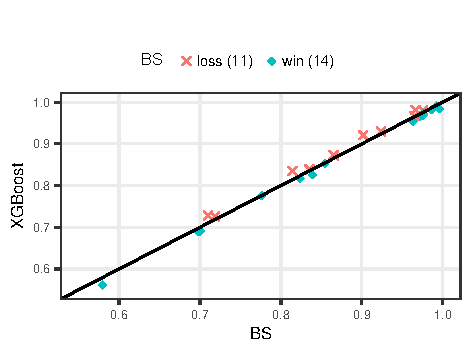
\includegraphics[width=.497\textwidth]{5_Guided_Search/fig/BS-Xgboost.pdf}
  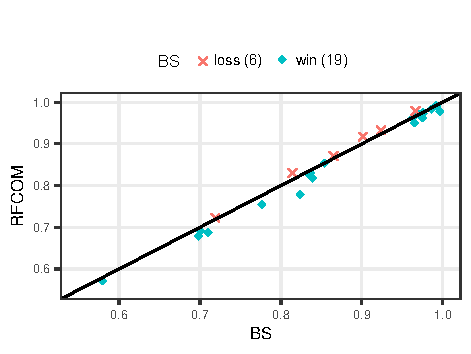
\includegraphics[width=.497\textwidth]{5_Guided_Search/fig/BS-RFCOM.pdf}\\
  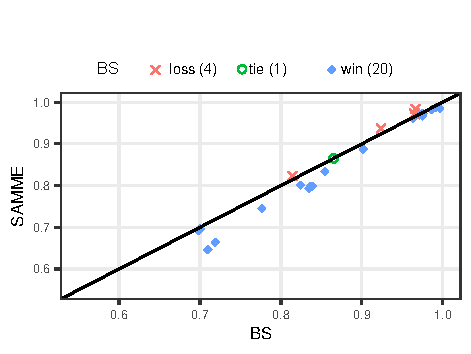
\includegraphics[width=.497\textwidth]{5_Guided_Search/fig/BS-SAMME.pdf}
  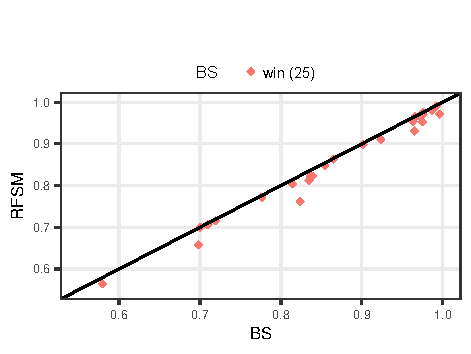
\includegraphics[width=.497\textwidth]{5_Guided_Search/fig/BS-RFSM.pdf}\\
  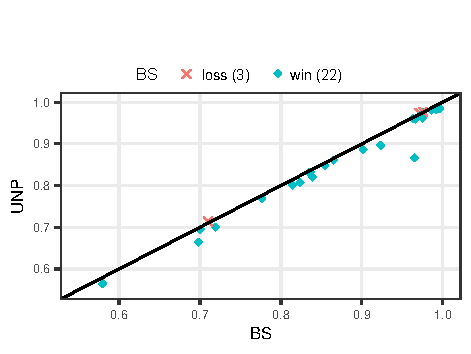
\includegraphics[width=.497\textwidth]{5_Guided_Search/fig/BS-UNP.pdf}
\end{center}
\caption{The performance of the proposed method against the defined ensembles NRD-NSE and RD-NSE.}
\label{BS-scatter}
\end{figure*}




\begin{figure*}[!ht]
\begin{center}\scriptsize
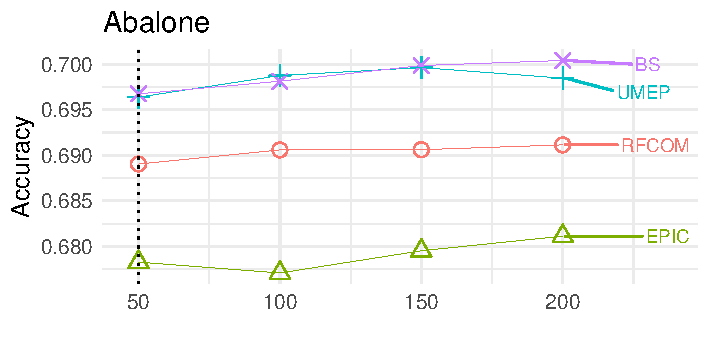
\includegraphics[width=.494\textwidth]{5_Guided_Search/fig/S-ENS-Abalone.pdf}
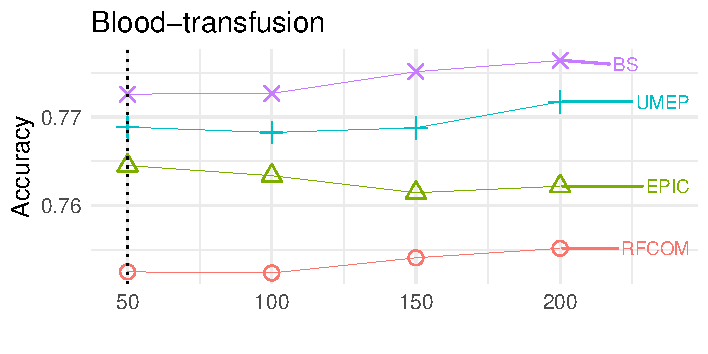
\includegraphics[width=.494\textwidth]{5_Guided_Search/fig/S-ENS-Blood-transfusion.pdf}\\
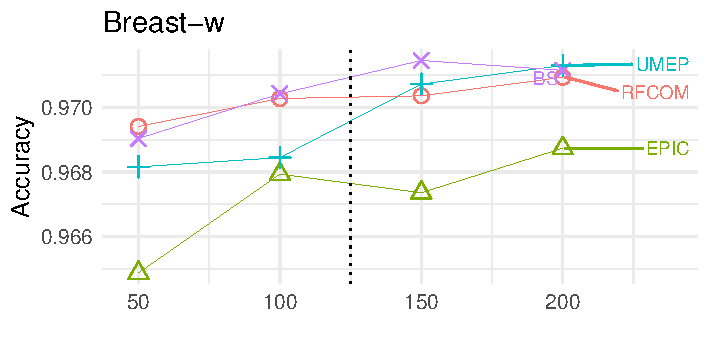
\includegraphics[width=.494\textwidth]{5_Guided_Search/fig/S-ENS-Breast-w.pdf} 
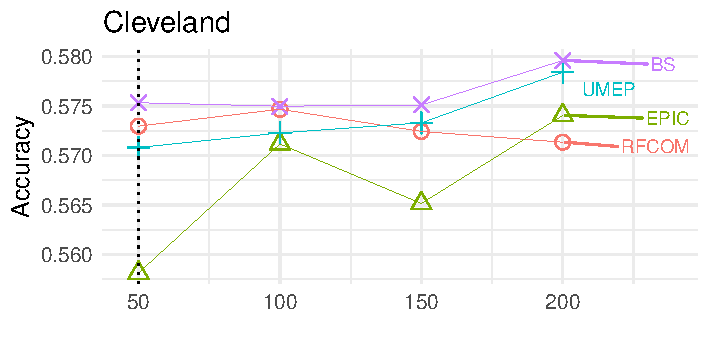
\includegraphics[width=.494\textwidth]{5_Guided_Search/fig/S-ENS-Cleveland.pdf}\\
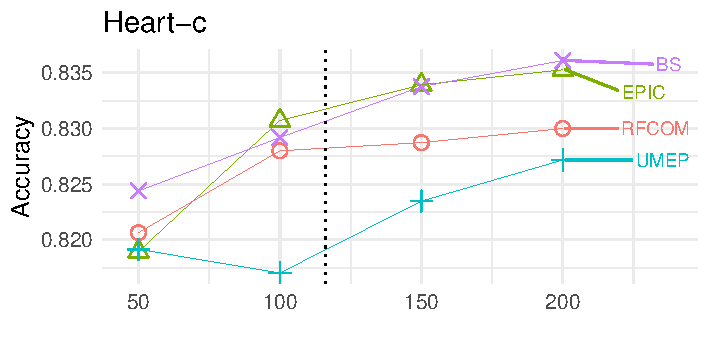
\includegraphics[width=.494\textwidth]{5_Guided_Search/fig/S-ENS-Heart-c.pdf}
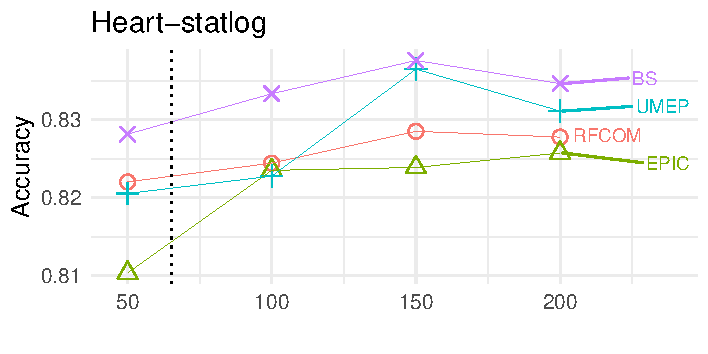
\includegraphics[width=.494\textwidth]{5_Guided_Search/fig/S-ENS-Heart-statlog.pdf}\\
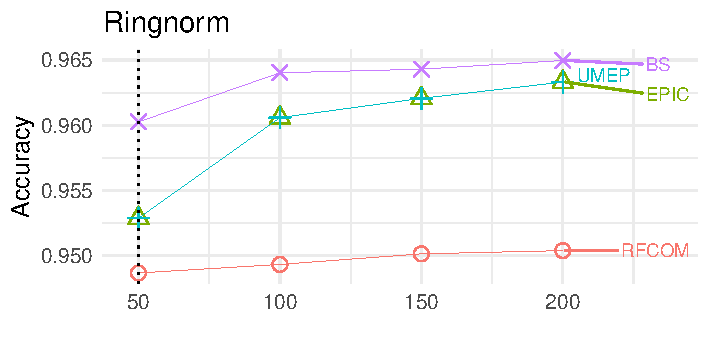
\includegraphics[width=.494\textwidth]{5_Guided_Search/fig/S-ENS-Ringnorm.pdf}
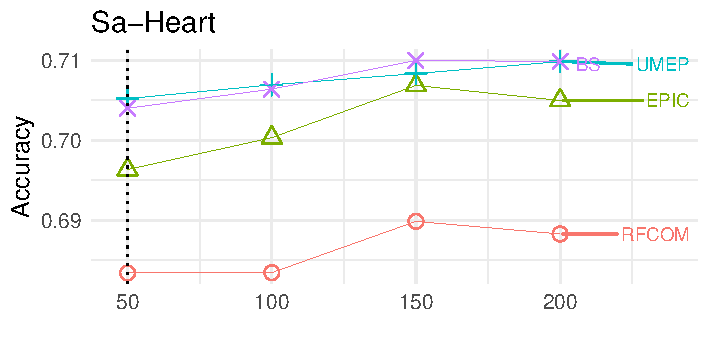
\includegraphics[width=.494\textwidth]{5_Guided_Search/fig/S-ENS-Sa-Heart.pdf}\\
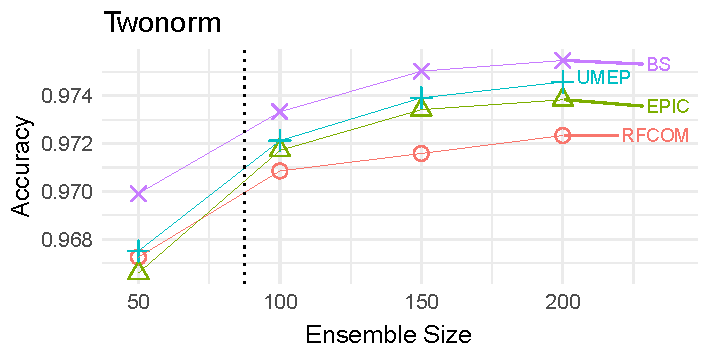
\includegraphics[width=.495\textwidth]{5_Guided_Search/fig/S-ENS-Twonorm.pdf}
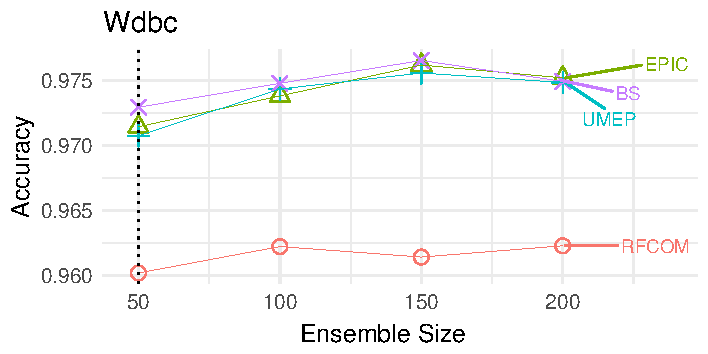
\includegraphics[width=.495\textwidth]{5_Guided_Search/fig/S-ENS-Wdbc.pdf}\\
\end{center}
\caption{The performance of ensemble pruning via guided search, a comparison with RFCOM, EPIC, and UMEP.}
\label{ch5:comparison.nonreduced}
\end{figure*}



It is interesting to analyze the performance of ensemble pruning via guided search for different ensemble sizes. This is important to check if its performance is consistent and not obtained due to randomness. Random Forest which is trained from whole training data, RFCOM, will be the baseline to compare against.  Figure \ref{ch5:comparison.nonreduced} shows the average accuracy of the pruned ensemble by (BS, UMEP, EPIC) and the unpruned one by RFCOM. Each point, in the figure, represents an average of 100 runs, and a percentage of $P=20\%$ is determined in advance to control the subensemble size. From Fig. \ref{ch5:comparison.nonreduced}, the behavior of BS dominates RFCOM according to both the accuracy and the ensemble size. Furthermore, the performance of BS over RFCOM can be reached, even, by pruning a low-size ensemble, the vertical dashed-line, regardless of what the size of RFCOM is. This shows how the proposed method can be an alternative to large-size ensembles, and a lot of computational resources could be saved by not overproducing models. However, this property could be different based on the classification task. We observe from Fig. \ref{ch5:comparison.nonreduced}, when EPIC and UMEP are ensembled together, via guided search, the subensemble realized a higher accuracy that was unreachable before. The statistical analysis will be discussed in Section \ref{statistical} to determine whether there is a significant improvement or not.







\subsection{Statistical Analysis}\label{statistical}
 To show if there is a significant improvement or not, Wilcoxon Signed Ranks Test \cite{wilcoxon1945} for pairwise comparison has been used. Table \ref{wilcoxontable} shows Wilcoxon Test \cite{wilcoxon1945} for the averages of the subensemble accuracy and subensemble size. The analysis from this table is as follows:
\begin{itemize}[nosep]
    \item[-] From the upper two parts (NRD-NSE, RD-NSE) which is a matrix 5 $\times$ 5: RFCOM significantly outperforms SAMME and RFSM by 90\% and 95\%, respectively. In addition, XGBoost is the best ensemble to learn from complete training data.
    \item[-] The proposed ensemble without pruning, UNP, is competitive with SAMME and RFCOM.
    
    \item[-] All RD-SE are significantly better than UNP in terms of accuracy and ensemble size, except FS and GA are only significantly better in terms of size. This proves the limitation of the proposed ensemble without pruning. 
    \item[-] HC and SA are comparable with UMEP, MDEP, and RFCOM in terms of accuracy, while HC and SA are significantly better in terms of subensemble size.
    \item[-] MDEP is comparable with RFCOM and UMEP in terms of accuracy. While it is better than RFCOM in terms of the ensemble size.
   
    \item[-] All RD-SE except FS and GA are comparable with XGBoost in terms of accuracy, while all RD-SE significantly outperform XGBoost in terms of ensemble size.  
    
     \item[-] BS is the only selection strategy under the proposed method that scores many ($\blacktriangle$). While it significantly outperforms the recent MDEP by 90\%.
     
    \item[-] In general, the lower part of Table \ref{wilcoxontable}, RD-SE,  includes subensembles with many ($\blacktriangle$) and many (\textbullet) where we have more flexibility to choose, according to the rigor of prediction and the computational resources.   
\end{itemize}

\vspace*{.3cm}
       

\begin{table*}[!ht]
\centering\scriptsize
\caption{Summary of the Wilcoxon test. Shape denotes the measure used, accuracy ($\blacktriangle$ $\triangle$) and size (\textbullet \textopenbullet). The filled shape ($\blacktriangle$ \textbullet) represents if the method in the row outperforms the one in the column or vice versa for ($\triangle$ \textopenbullet). Upper diagonal of level significance $\alpha=0.9$, lower diagonal level of significance $\alpha=0.95$.}

\resizebox{\textwidth}{!}{\begin{tabular}{|c
|l|c|c|c|c|c|c|c|c|c|c|c|c|c|c|}
\hline
& &(1) &(2) &(3) &(4) &(5) &(6) &(7) &(8) &(9) &(10) &(11) &(12)& (13)& (14) \\
\hline
\multirow{3}{*}{ NRD-NSE} & XGBoost(1) & - -& $\blacktriangle$ & $\blacktriangle$ & $\blacktriangle$ & $\blacktriangle$ & \textopenbullet & \textopenbullet  &\textopenbullet & $\blacktriangle$ \textopenbullet  &  \textopenbullet& \textopenbullet & \textopenbullet& \textopenbullet & $\blacktriangle$ \textopenbullet  \\
\cline{2-16}
 & SAMME(2) & $\triangle$ &- -& $\triangle$ &  &  & $\triangle$ \textopenbullet& $\triangle$ \textopenbullet &$\triangle$ \textopenbullet & \textopenbullet & $\triangle$ \textopenbullet & $\triangle$ \textopenbullet & $\triangle$  \textopenbullet& $\triangle$ \textopenbullet &  \textopenbullet \\
\cline{2-16}
&RFCOM (3)& $\triangle$ &  &- -& $\blacktriangle$ &  & \textopenbullet & $\triangle$ \textopenbullet &  \textopenbullet & $\blacktriangle$ \textopenbullet& $\triangle$\textopenbullet &  \textopenbullet &\textopenbullet  & \textopenbullet & \textopenbullet \\
\hline
\multirow{2}{*}{RD-NSE} &RFSM (4)&$\triangle$ &  & $\triangle$ &- -&  & $\triangle$ \textopenbullet & $\triangle$ \textopenbullet & $\triangle$ \textopenbullet & $\blacktriangle$ \textopenbullet & $\triangle$ \textopenbullet & $\triangle$ \textopenbullet & $\triangle$ \textopenbullet & $\triangle$ \textopenbullet & \textopenbullet  \\
\cline{2-16}
&UNP (5)&$\triangle$ &  &  &  &- -& $\triangle$ \textopenbullet & $\triangle$ \textopenbullet &$\triangle$ \textopenbullet &\textopenbullet & $\triangle$ \textopenbullet & $\triangle$ \textopenbullet  & $\triangle$ \textopenbullet & $\triangle$ \textopenbullet &  \textopenbullet \\
\hline
\multirow{8}{*}{RD-SE} &EPIC (6)& \textbullet& $\blacktriangle$\textbullet & \textbullet & $\blacktriangle$ \textbullet & $\blacktriangle$ \textbullet &- -& $\triangle$ &$\triangle$ &$\blacktriangle$ \textopenbullet & $\triangle$ \textbullet & $\triangle$ \textopenbullet & \textopenbullet & \textopenbullet & $\blacktriangle$ \textopenbullet \\
\cline{2-16}
&UMEP (7)&\textbullet & $\blacktriangle$ \textbullet & \textbullet  & $\blacktriangle$ \textbullet & $\blacktriangle$ \textbullet &$\blacktriangle$  &- -&  & $\blacktriangle$ \textopenbullet & $\triangle$ \textbullet &\textopenbullet  & \textopenbullet & $\blacktriangle$ \textopenbullet & $\blacktriangle$ \textopenbullet \\
\cline{2-16}
& MDEP(8) &\textbullet  & $\blacktriangle$\textbullet&  \textbullet&$\blacktriangle$ \textbullet  &$\blacktriangle$ \textbullet&$\blacktriangle$  &   &- -&$\blacktriangle$ \textopenbullet &$\triangle$  \textbullet& \textopenbullet & \textopenbullet & \textopenbullet  &$\blacktriangle$ \textopenbullet   \\
\cline{2-16}
&FS (9)& $\triangle$ \textbullet & \textbullet & $\triangle$ \textbullet & $\triangle$ \textbullet  & \textbullet  & $\triangle$ \textbullet & $\triangle$ \textbullet& $\triangle$ \textbullet &- -& $\triangle$ \textbullet & $\triangle$ \textbullet & $\triangle$ \textbullet & $\triangle$ \textbullet & $\triangle$ \textbullet \\
\cline{2-16}
&BS (10)& \textbullet& $\blacktriangle$ \textbullet & $\blacktriangle$ \textbullet & $\blacktriangle$ \textbullet & $\blacktriangle$ \textbullet & $\blacktriangle$ \textopenbullet& $\blacktriangle$ \textopenbullet & \textopenbullet & $\blacktriangle$ \textopenbullet &- -& $\blacktriangle$ \textopenbullet & $\blacktriangle$ \textopenbullet & $\blacktriangle$ \textopenbullet & $\blacktriangle$ \textopenbullet \\
\cline{2-16}
&HC (11)& \textbullet& $\blacktriangle$ \textbullet & \textbullet & $\blacktriangle$ \textbullet & $\blacktriangle$ \textbullet &$\blacktriangle$ \textbullet  & \textbullet &\textbullet & $\blacktriangle$ \textopenbullet & $\triangle$ \textbullet &- -&  & $\blacktriangle$ \textopenbullet & $\blacktriangle$ \textopenbullet \\
\cline{2-16}
&SA (12) & \textbullet& $\blacktriangle$ \textbullet & \textbullet & $\blacktriangle$ \textbullet & $\blacktriangle$ \textbullet & \textbullet  & \textbullet & \textbullet & $\blacktriangle$ \textopenbullet & $\triangle$ \textbullet&  &- -& $\blacktriangle$ \textopenbullet& $\blacktriangle$ \textopenbullet \\
\cline{2-16}
&BGWO (13) & \textbullet& $\blacktriangle$ \textbullet &  \textbullet & $\blacktriangle$ \textbullet & $\blacktriangle$ \textbullet& \textbullet  & $\triangle$ \textbullet &  \textbullet &$\blacktriangle$ \textopenbullet & $\triangle$ \textbullet& $\triangle$ \textbullet  &  \textbullet &- -& $\blacktriangle$ \textopenbullet\\
\cline{2-16}
&GA (14) & $\triangle$ \textbullet& \textbullet & \textbullet & \textbullet &  \textbullet & $\triangle$ \textbullet& $\triangle$ \textbullet &$\triangle$ \textbullet & $\blacktriangle$\textopenbullet & $\triangle$  \textbullet& $\triangle$ \textbullet  & $\triangle$ \textbullet& $\triangle$ \textbullet&- -\\
\hline
\end{tabular}}
\label{wilcoxontable}
\end{table*}



\afterpage{
\begin{landscape}
\begin{table}[!ht]
        \centering \scriptsize
\caption{Average accuracy and standard deviation of the proposed method with and without instance selection, ensemble size $T= 200$, $P$=20\%. The best value is in bold, while the second best is underlined.}
\label{wIS-complete-table}
\renewcommand{\arraystretch}{1.3}
\begin{adjustbox}{max width=1.5\textwidth} \begin{tabular}{llccccccccccccccc}
  \hline
   & & \multicolumn{5}{c}{Without Instance Selection}&\multicolumn{5}{c}{Instance Selection (Proposed)}\\
 \cmidrule(lr){3-7} \cmidrule(lr){8-12} 
 \#&  Dataset &  wIS-UNP & wIS-EPIC & wIS-UMEP & wIS-MDEP & \multicolumn{1}{c}{wIS-BS} & \multicolumn{1}{c}{UNP} & \multicolumn{1}{c}{EPIC} & \multicolumn{1}{c}{UMEP} &
 \multicolumn{1}{c}{MDEP} &
 \multicolumn{1}{c}{BS} \\ 
\hline
$D_1$ & Abalone &  \textbf{70.41$\pm$1.02}  & 69.31 $\pm$ 1.00  & 69.56 $\pm$ 1.14  & 69.48 $\pm$ 1.08  & 69.47 $\pm$ 1.08  &  69.52 $\pm$ 0.64 & 68.11 $\pm$ 1.80 & 69.85 $\pm$ 1.00 & 69.96 $\pm$ 1.12   & \underline{70.04 $\pm$ 1.14}\\ 

  $D_2$ & Australian &  87.00$\pm$ 3.10  & \textbf{87.18 $\pm$ 2.92}  & 86.89 $\pm$ 2.93  & 87.13 $\pm$ 2.91  & \underline{87.14 $\pm$ 2.88}  & 86.05 $\pm$ 2.46 & 85.47 $\pm$ 2.62 & 86.43 $\pm$ 2.65 & 86.25 $\pm$ 2.80 &  86.50 $\pm$ 2.60 \\ 
  
  $D_3$ & Blood-transfusion &  \underline{77.24$\pm$ 1.38}  & 77.20 $\pm$ 2.16  & 76.92 $\pm$ 2.14 & 77.19 $\pm$ 2.09   & 77.03 $\pm$ 2.10 &  76.90 $\pm$ 1.45 & 76.22 $\pm$ 3.65 & 77.17 $\pm$ 2.08 &77.22 $\pm$ 2.08  & \textbf{77.64 $\pm$ 2.22}\\ 
  
  $D_4$ & Breast-w &  \underline{97.25$\pm$ 1.43} & 96.96 $\pm$ 1.56 & 97.17 $\pm$ 1.41 & 97.19 $\pm$ 1.48	  & 97.20 $\pm$ 1.47
 &   \textbf{97.42 $\pm$ 1.17}  & 96.87 $\pm$ 1.30 & 97.13 $\pm$ 1.25 &97.13 $\pm$ 1.31   & 97.12 $\pm$ 1.23  \\ 
  
  $D_5$ & Cleveland &  57.47$\pm$ 3.04  & 57.58 $\pm$ 3.46 & 57.43 $\pm$ 3.08  & 57.60 $\pm$ 3.02  & 57.40 $\pm$ 3.57  &  56.50 $\pm$ 2.88 &57.41 $\pm$ 4.27 & \underline{57.84 $\pm$ 3.12} & 57.56 $\pm$ 3.10 & \textbf{57.96 $\pm$ 3.66} \\ 
  
  $D_6$ & Dermatology &  97.75$\pm$ 1.45  & 97.86 $\pm$ 1.58  & \textbf{97.93 $\pm$ 1.47}  & \textbf{97.93 $\pm$  1.49}	 & \underline{97.92 $\pm$ 1.47}
  &  97.46 $\pm$ 1.65 & 97.32 $\pm$ 1.89 & 97.56 $\pm$ 1.62 & 97.63 $\pm$ 1.65  & 97.53 $\pm$ 1.72 \\ 
  
  $D_7$ & Diabetic &  \textbf{71.08$\pm$ 2.79}  & 68.64 $\pm$ 2.46  & 68.68 $\pm$ 2.52  & 68.71 $\pm$  2.33  & 68.59 $\pm$ 2.44  &  66.38 $\pm$ 2.94 & 69.63 $\pm$ 2.75  & 70.26 $\pm$ 3.20 &\underline{70.49 $\pm$ 3.00}& 69.81 $\pm$ 3.10 \\ 
  
  $D_8$ & Heart-c &  \textbf{84.02 $\pm$ 4.38} & 82.65 $\pm$ 4.28 & 82.64 $\pm$ 4.19  & 82.60 $\pm$ 4.17  & 82.97 $\pm$ 4.05 &  83.22 $\pm$ 4.49 & 83.53 $\pm$ 4.25 & 82.72 $\pm$ 4.58 & 83.12 $\pm$ 4.33 & \underline{83.61 $\pm$ 4.26}\\ 
  
  $D_9$ & Heart-statlog &  \textbf{83.98$\pm$ 4.09} & 82.69 $\pm$ 4.13 & 82.50 $\pm$ 4.45 & 82.83 $\pm$ 4.28  & 82.72 $\pm$ 4.26 & 83.07 $\pm$ 4.71 & 82.57 $\pm$ 4.45 & 83.11 $\pm$ 4.07 &\underline{83.70 $\pm$ 4.26}&  83.46 $\pm$ 4.27 \\ 
  
  $D_{10}$ & Ionosphere &  93.32$\pm$ 2.98  & 93.85 $\pm$ 2.77 &  \textbf{93.96 $\pm$ 2.67}  & \underline{93.93 $\pm$ 2.79}   & \underline{93.93 $\pm$ 2.76} & 89.67 $\pm$ 2.98 & 92.41 $\pm$ 2.61  & 91.93 $\pm$ 2.89 &92.49 $\pm$ 2.74&  92.34 $\pm$ 2.75 \\ 
  
  $D_{11}$ & Led24 &  \underline{71.99 $\pm$ 1.61}  & 70.37 $\pm$ 1.78  & \textbf{72.04 $\pm$ 1.47} & 69.84 $\pm$ 2.67  & 67.84 $\pm$ 2.82 &  70.02 $\pm$ 1.76 & 71.75 $\pm$ 1.46 & 71.78 $\pm$ 1.45 & 68.66 $\pm$ 3.79&  71.89 $\pm$ 1.45 \\ 
  
  $D_{12}$ & Mammographic &  82.85 $\pm$ 2.67  & 83.32 $\pm$ 2.63	  & 83.57 $\pm$ 2.13	 & 83.66 $\pm$ 2.21	& 83.84 $\pm$ 2.34
 & 82.06 $\pm$ 2.51 & 83.37 $\pm$ 2.64 & \underline{84.00 $\pm$ 2.32} &\textbf{84.05 $\pm$ 2.27}& 83.89 $\pm$ 2.36 \\ 
  
  $D_{13}$ & Mfeat-fourier &  82.81 $\pm$ 1.44  & 83.24 $\pm$ 1.32  & 83.32 $\pm$ 1.40 & \textbf{83.48 $\pm$ 1.42}  & \underline{83.38 $\pm$ 1.48}  & 80.14 $\pm$ 1.50 & 80.89 $\pm$ 1.65 & 81.34 $\pm$ 1.56 &81.12 $\pm$ 1.63 &  81.41 $\pm$ 1.62 \\ 
  
  $D_{14}$ & Mfeat-karh &  \textbf{96.80$\pm$ 0.86} & 95.82 $\pm$ 0.83	  & 95.84 $\pm$ 0.86 & 95.98 $\pm$ 0.89  & 95.96 $\pm$ 0.86 & 96.13 $\pm$ 0.88 & 96.19 $\pm$ 0.86 & 96.27 $\pm$ 0.85 &96.28 $\pm$ 0.96 &\underline{96.31 $\pm$ 0.89} \\ 
  
  $D_{15}$ & Mfeat-zernike &  80.06$\pm$ 1.22  & 78.15 $\pm$ 1.48  & 78.83 $\pm$ 1.35 & 79.37 $\pm$ 1.39  & 78.89 $\pm$ 1.37  &  80.72 $\pm$ 1.24 & 82.19 $\pm$ 1.52 & \textbf{82.48 $\pm$ 1.44} &82.20 $\pm$ 1.41 &\underline{ 82.38 $\pm$ 1.39} \\ 
  
  $D_{16}$ & Optdigits &  98.29$\pm$ 0.35 & 98.79 $\pm$ 0.33 & \underline{98.80 $\pm$ 0.32}  & \underline{98.80 $\pm$ 0.32}  & \textbf{98.81 $\pm$ 0.32}  &  98.09 $\pm$ 0.38 & 98.61 $\pm$ 0.31 & 98.60 $\pm$ 0.31 &98.59 $\pm$ 0.30 & 98.61 $\pm$ 0.32 \\ 
  
  $D_{17}$ & Penbased &  98.31$\pm$ 0.27 & \textbf{99.32 $\pm$ 0.16}	 & 99.30 $\pm$ 0.17 & 99.29 $\pm$  0.17 & \underline{99.31 $\pm$ 0.16}  &  98.22 $\pm$ 0.27 & 99.21 $\pm$ 0.16 & 99.19 $\pm$ 0.17 &99.10 $\pm$ 0.69 &  99.20 $\pm$ 0.16  \\ 
  
  $D_{18}$ & Ringnorm &  \textbf{96.66$\pm$ 0.46}  & 96.62 $\pm$ 0.47 & 96.64 $\pm$ 0.49 & 96.64 $\pm$ 0.49  & \underline{96.65 $\pm$ 0.47}  &  86.69 $\pm$ 1.15 & 96.33 $\pm$ 0.51 & 96.33 $\pm$ 0.51 & 96.37 $\pm$ 0.49 &  96.50 $\pm$ 0.48 \\ 
  
  $D_{19}$ & Sa-heart &  71.23$\pm$ 3.38 & 69.06 $\pm$ 3.56	 & 69.13 $\pm$ 3.56 & 69.44 $\pm$ 3.39  & 69.35 $\pm$ 3.19
 & \textbf{71.41 $\pm$ 3.77} & 70.50 $\pm$ 4.30 & 70.98 $\pm$ 3.86 & \underline{71.25 $\pm$ 3.65} & 70.98 $\pm$ 4.06 \\ 
  
  $D_{20}$ & Satimage &  89.45$\pm$ 0.74  & 91.33 $\pm$ 0.73  & 91.33 $\pm$ 0.73 & \underline{91.34 $\pm$ 0.72}   & \textbf{91.39 $\pm$ 0.75}
 & 88.70 $\pm$ 0.78 & 90.17 $\pm$ 0.75 & 90.05 $\pm$ 0.77 & 89.81 $\pm$ 1.39 &  90.16 $\pm$ 0.72  \\
 
  $D_{21}$ & Segment &  96.87$\pm$ 0.89	 & \textbf{98.05 $\pm$ 0.68}  & 98.00 $\pm$ 0.68 & 98.01 $\pm$ 0.69 & \underline{98.03 $\pm$ 0.65}  &  95.94 $\pm$ 0.90 & 96.61 $\pm$ 0.77 & 96.54 $\pm$ 0.74 & 96.51 $\pm$ 0.87 & 96.61 $\pm$ 0.77  \\ 
  
  $D_{22}$ & Texture &  98.80$\pm$ 0.33	  & \textbf{99.71 $\pm$ 0.17} & \textbf{99.71 $\pm$ 0.17} & \textbf{99.71 $\pm$ 0.17}  & \textbf{99.71 $\pm$ 0.17} &  98.40 $\pm$ 0.35 & \underline{99.63 $\pm$ 0.19} & \underline{99.63 $\pm$ 0.19} &\underline{99.63 $\pm$ 0.16} & \underline{99.63 $\pm$ 0.18} \\ 
  
  $D_{23}$ & Twonorm &  \textbf{97.69$\pm$ 0.36}	  & 96.61 $\pm$ 0.45 & 96.62 $\pm$ 0.44  & 96.62 $\pm$ 0.44   & 96.68 $\pm$  0.41 & \textbf{ 97.69 $\pm$ 0.37}& 97.38 $\pm$ 0.39 & 97.46 $\pm$ 0.38 &97.47 $\pm$ 0.42 &\underline{ 97.55 $\pm$ 0.35} \\ 
  
  $D_{24}$ & Waveform &  \textbf{85.66 $\pm$ 1.04}	 & 84.42 $\pm$ 1.11	 & 84.39 $\pm$ 1.15  & 84.40 $\pm$ 1.17  & 84.46 $\pm$ 1.11
  &  84.87 $\pm$ 1.16 & 84.59 $\pm$ 1.00 & 85.41 $\pm$ 0.95 &85.34 $\pm$ 1.07 & \underline{85.42 $\pm$ 0.93} \\ 
  
  $D_{25}$ & Wdbc &  96.81$\pm$ 1.44  & \underline{97.57 $\pm$ 1.21}  & 97.46 $\pm$ 1.29  & 97.56 $\pm$ 1.22  & \textbf{97.66 $\pm$ 1.16} &  96.17 $\pm$ 1.85 & 97.52 $\pm$ 1.46 & 97.48 $\pm$ 1.63 &97.34 $\pm$ 1.58 & 97.49 $\pm$ 1.56 \\ 
  
   \hline
  \multicolumn{2}{c}{\textbf{AR-Friedman}}& \multicolumn{1}{c}{\textbf{4.3}} &\multicolumn{1}{c}{5.76}&\multicolumn{1}{c}{5.6} &\multicolumn{1}{c} {4.84} &\multicolumn{1}{c}{4.88} &\multicolumn{1}{c} {7.54} & \multicolumn{1}{c}{6.84}& \multicolumn{1}{c}{5.44} &\multicolumn{1}{c}{5.4} &\multicolumn{1}{c}{\underline{4.4}}  \\ 
\hline
\end{tabular}
\end{adjustbox}
\end{table}
\end{landscape}
}


\subsection{Validation of the Methodology}
We have shown the superiority of the proposed ensemble in the previous sections. However, it is necessary to validate its components (instance selection, proposed ensemble, and guided search-based pruning). Thus, we performed additional experiments to validate our method.  

\textit{The effect of instance selection to the constructed ensemble}, we compared the obtained results without instance selection (wIS) and with instance selection (proposed). Table \ref{wIS-complete-table} shows the complete results of the 25 datasets. The worst average rank via Friedman Test \cite{demsar2006} is scored by UNP. Hence, coupling instance selection with the unpruned proposed ensemble has a limited accuracy in comparison with wIS-UNP. This means that IS contributed to form simpler, less space complexity, ensembles rather than more accurate ensembles. Table \ref{wIS-wilcoxon-table} shows the Wilcoxon Test \cite{wilcoxon1945} for the results from Table \ref{wIS-complete-table}. The results confirm that the proposed ensemble without pruning, UNP, is not effective. However, it is comparable with ensembles that are trained from whole training data, RFCOM and SAMME.

\textit{The validation of the proposed ensemble}, we show how the proposed ensemble, Section \ref{proposed.mcs}, is effective. Table \ref{wIS-wilcoxon-table} confirms that wIS-UNP which uses the same amount of training data is significantly better than SAMME and RFCOM at a 95\% confidence level. Furthermore, there is no ensemble, among the thirteen models, that is significantly higher than wIS-UNP.   


\textit{The validation of guided search-based pruning}, we prove how guided search is more effective whether an instance selection is applied or not. From Table \ref{wIS-wilcoxon-table}, when instance selection is performed, BS shows a significant difference at a 95\% confidence level better than EPIC and UMEP. In addition, MDEP is significantly worse than BS at a 90\% confidence level. Moreover, BS is able to compensate for the error of UNP, confirmed by the significant difference between BS and RFCOM. Without applying instance selection, wIS-BS is still outperforming wIS-EPIC and wIS-UMEP at a 95\% confidence level. This shows the limited performance of the existing pruning methods in comparison with the proposed guided search-based pruning. 


As a summary, with the experiments of this section. We have separately validated the different parts of our method, showing their usefulness. We proved that simpler and better ensembles could be properly designed when all the parts are used together.  
\vspace*{.3cm}

\begin{table}[!ht]
\centering\scriptsize
\caption{Summary of the Wilcoxon test. $\blacktriangle$ = the method in the row improves the method of the column. $\triangle$ = the method in the column improves the method of the row. Upper diagonal of level significance $\alpha=0.9$, Lower diagonal level of significance $\alpha=0.95$}
\label{wIS-wilcoxon-table}
{\begin{tabular}{
|l|c|c|c|c|c|c|c|c|c|c|c|c|c|}
\hline
&(1) &(2) &(3) &(4) &(5) &(6) &(7) &(8) &(9) &(10) &(11) &(12) &(13) \\
\hline
XGBoost (1)& -& $\blacktriangle$ & $\blacktriangle$ &  &  &  &  &  & $\blacktriangle$ &  &  &  &  \\
\hline
SAMME (2)& $\triangle$ & -& $\triangle$ & $\triangle$ & $\triangle$ & $\triangle$ & $\triangle$ & $\triangle$ &  & $\triangle$ & $\triangle$ & $\triangle$ & $\triangle$ \\
\hline
RFCOM (3)& $\triangle$ &  & -& $\triangle$ & $\triangle$ & $\triangle$ & $\triangle$ & $\triangle$ &  &  & $\triangle$ &  & $\triangle$ \\
\hline
wIS-UNP (4)&  & $\blacktriangle$ & $\blacktriangle$ & -&  &  &  &  & $\blacktriangle$ & $\blacktriangle$ &  &  &  \\
\hline
wIS-EPIC (5)&  & $\blacktriangle$ &  &  & -&  & $\triangle$ & $\triangle$ & $\blacktriangle$ &  &  &  &  \\
\hline
wIS-UMEP (6)&  & $\blacktriangle$ & $\blacktriangle$ &  &  & -& $\triangle$ & $\triangle$ & $\blacktriangle$ &  &  &  &  \\
\hline
wIS-MDEP (7)&  & $\blacktriangle$ & $\blacktriangle$ &  & $\blacktriangle$ & $\blacktriangle$ & -&  & $\blacktriangle$ &  &  &  &  \\
\hline
wIS-BS (8)&  & $\blacktriangle$ & $\blacktriangle$ &  & $\blacktriangle$ & $\blacktriangle$ &  & -& $\blacktriangle$ &  &  &  &  \\
\hline
UNP (9)& $\triangle$ &  &  & $\triangle$ &$\triangle$ & $\triangle$ & $\triangle$ &  & -& $\triangle$ & $\triangle$ & $\triangle$ & $\triangle$ \\
\hline
EPIC (10)&  & $\blacktriangle$ &  &  &  &  &  &  & $\blacktriangle$ & -& $\triangle$ & $\triangle$ & $\triangle$ \\
\hline
UMEP (11)&  & $\blacktriangle$ &  &  &  &  &  &  & $\blacktriangle$ & $\blacktriangle$ & -&  & $\triangle$ \\
\hline
MDEP (12)&  & $\blacktriangle$ &  &  &  &  &  &  & $\blacktriangle$ & $\blacktriangle$ &  & -& $\triangle$ \\
\hline
BS (13)&  & $\blacktriangle$ & $\blacktriangle$ &  &  &  &  &  & $\blacktriangle$ & $\blacktriangle$ & $\blacktriangle$ &  & -\\
\hline
\end{tabular}}
\end{table}





\subsection{Advantages of the proposed method}

Among the advantages of the proposed method are: (1) The instance selection method is applied only once from the whole training data. (2) The individual models are independent, and the generation step could be accelerated by a parallel implementation. (3) The reduced data helps to generate less complex models with a fast prediction time. (4) The guided search preserves promising search areas to identify a subensemble properly. (5) The proposed methodology proved its capability to maximize learning from the reduced data. Regarding that, it can be used to improve the precision of IS method. (6) The ease of implementation with wide flexibility to apply different IS methods and different classifier types.



\subsection{Time Complexity} \label{complex}
The classification speed as determined in \citep{martinez2009} mainly depends on (1) the ensemble size and (2) the complexity of individual classifiers. While Table \ref{complecity} summarize the time complexity of the applied ensemble pruning methods. For GA \& BGWO, ($\hat P$) represents population size, and ($E$) represents the number of epochs. While $\hat{T}$ denotes the size of the preselected classifiers, \textit{New subset in Fig. \ref{topology}}, that is formed by both EPIC \& UMEP.
\vspace*{.3cm}

\begin{table}[!ht]
\centering
 \caption{Time complexity of ensemble selection}
\label{complecity}
\renewcommand{\arraystretch}{1}
\begin{adjustbox}{max width=1\textwidth}
\begin{tabular}{l|l}
\hline
Ensemble selection & Time complexity\\ \hline
MDEP & $\mathcal{O}( T \cdot  \log{T})$\\
UMEP & $\mathcal{O}(T \cdot N) \rightarrow$  \circled{1}\\
EPIC & $\mathcal{O}( T \cdot\log{T}) \rightarrow$ \circled{2}\\
FS \& BS   &\circled{1}+\circled{2}+ $\mathcal{O}({\hat{T}}^3)$\\
HC - SA & \circled{1}+\circled{2}+ $\mathcal{O}( \hat{T} \cdot N \cdot M)$ \\
GA - BGWO & \circled{1}+\circled{2}+ $\mathcal{O}(E \cdot \hat P \cdot \hat{T} \cdot N \cdot M)$\\
\hline
\end{tabular}
\end{adjustbox}
\end{table}
  